\documentclass{article}

% Formatting
\usepackage[utf8]{inputenc}
\usepackage[margin=1in]{geometry}
\usepackage[titletoc,title]{appendix}

\usepackage{amsmath,amsfonts,amssymb,mathtools, amsthm}

\usepackage{graphicx,float}

\usepackage[ruled,vlined]{algorithm2e}
\usepackage{algorithmic}

\usepackage{float}

\usepackage{caption}
\usepackage{subcaption}

% Code syntax highlighting
% https://www.overleaf.com/learn/latex/Code_Highlighting_with_minted
\usepackage{minted}
\usemintedstyle{borland}

% References
% https://www.overleaf.com/learn/latex/Bibliography_management_in_LaTeX
% https://en.wikibooks.org/wiki/LaTeX/Bibliography_Management
\usepackage{biblatex}
\addbibresource{references.bib}

% Title content
\title{AMATH 482 A1: A Submarine Problem}
\author{Rishabh Verma}
\date{January 27, 2021}

\begin{document}

\maketitle

% Abstract
\begin{abstract}
    This paper contains the analysis of 3-D spatial-domain data where each point indicates the acoustic pressure measured at the corresponding coordinate in the Puget Sound. There exists a mysterious submarine emitting an unknown frequency through the waters. Using digital signal processing techniques, I identify this submarine's sonic signature and determine its path through the Puget Sound. These mechanisms can be easily re-applied in the future to locate any other submarine of the same class at any time.
\end{abstract}

% Introduction and Overview
\section{Introduction and Overview}
A submarine of unknown class is suspected to be in the Puget Sound. There exists audio equipment which can record the acoustic pressure across an evenly spaced 64x64x64 lattice within the Puget Sound. This lattice exists within a 20x20x20 region of unknown physical distance units (pdu's). The actual distance unit does not matter because the goal is to identify the submarine's acoustic signature and trajectory; this can all be given in terms of pdu.

Our data includes 49 snapshots of Puget Sound acoustics taken over a 24-hour span at half-hour increments in time. Each snapshot contains the submarine's acoustic signature as well as a considerable amount of noise. If the noise can be removed, the acoustic signature should look like a wavefront where the strongest displacement is observed by the location of the submarine, and the wavefront's amplitude decays with increasing distance from this maximum. Thus, the filtered data point with maximum amplitude will make a good estimate for the location of the submarine.

\subsection{Deliverables}

To re-iterate, the expected items to be computed are

\begin{itemize}
	\item the spatial frequency emitted by the submarine
	\item the trajectory of the submarine
	\end{itemize}

In order to obtain these, the first item requires denoising the spectrum of the data. The second item requires denoising the data itself in the spatial domain. The methods used for this will rely on applying the Discrete Fourier Transform (DFT) and its inverse. 

%  Theoretical Background
\section{Theoretical Background}

\subsection{Spatial acoustic data}

An acoustic waveform is commonly understood as a sinusoidal displacement function in terms of time. However, an acoustic waveform can also be understood as a sinusoidal displacement function in terms of space. Suppose there exists a point source at $x=0$ which emits a signal of wavelength $4$, and that this signal does not decay with respect to distance. At some instant in time, the reading of acoustic sensors at $x=1, 2, 3, 4$ might read 

\begin{equation}
\begin{bmatrix}
x_1&x_2&x_3&x_4
\end{bmatrix}=\begin{bmatrix}
	1&0&-1&0
\end{bmatrix}
\label{eqn:spatial}
\end{equation}

in which the RHS sensor values, though dependent on the instantaneous phase of the signal source, indicate a single oscillation. Realistically, a point source of a 3-dimensional acoustic pressure wave will emit a signal whose strength is inversely proportional to the square of the distance. For our purposes, we only need to understand that the signal's amplitude decays with respect to distance from the point source. 


\subsubsection{An analogy}
The notion of recording acoustic pressure but working with spatial data can be disorienting. For this, I offer an analogy. Suppose a researcher by a pond has a device which can freeze time. She walks on the dock, drops a stone into the water, freezes time, and writes down the vertical displacement of the water across a horizontal grid of points. This is an instantaneous 2-dimensional measurement of a longitudinal pressure signal across a lattice of points, and is analogous to our submarine data, though with one dimension lesser. The period of the measured signal is exactly the wavelength of the pressure wave in water.


\subsection{Analyzing the Fourier spectrum of spatial data}
\subsubsection{Output of the Discrete Fourier Transform}

%Consider a discrete signal with $N$ points. The method of Discrete Fourier Transform allows us to determine how well this signal fits oscillations of various frequencies. These oscillations can be easily characterized by their wavelength. For example, the oscillation corresponding to the $k=1$ bin has a wavelength equal to $N$ samples, and so one wavelength of such an oscillation fits within the signal domain. The oscillation corresponding to the $k=2$ bin has a wavelength equal to $N/2$ samples, and so two of these wavelengths fit within the domain. %TODO do I need to justfiy any maths?
%The magnitude of these bins ranges from $|k|=0$ to $|k|=N/2$, where the greatest observable frequency has a wavelength of $N/|k| = N/(N/2) = 2$, and can fit $N/2$ wavelengths across the domain.
%
%\subsubsection{Finding the signal in clean spatial data}
The submarine emits a signal which should ideally appear as a periodic spherical wavefront. If an oscillation has fixed period $x$ pdu, it will have fixed spatial frequency $1/x$ pdu$^{-1}$.

Because the data divides a 20x20x20 physical region into a 64x64x64 lattice, the physical coordinate corresponding to a value at index $(x^*,y^*,z^*)$ can be obtained with a linear interpolation from $-10$ to $10$ with $64$ points. This is given by dropping the final point off of MATLAB's \texttt{linspace(-20,20,65)}. Note that if \texttt{linspace(-20,20,64)} is used instead, then the physical locations will not be centered at zero.

The $k$-th frequency bin outputted by the DFT corresponds to a wave which is periodic on the domain and includes $k$ oscillations. Such a wave has period $D/k$. 

Consider a wave $\sin(2\pi fx)$ with frequency $f$ and spatial parameter $x$. Its period is $\dfrac{1}{f}$, and its natural frequency is $\omega = 2\pi f$. 

In the DFT, all oscillations must be periodic by integer order. The $k$-th bin contains a wave with $k$ oscillations over a domain of width $D=20$, and so it has period $\dfrac{D}{k}=\dfrac{20}{k}$. This means it has frequency $\dfrac{k}{20}$ and natural frequency $2\pi\dfrac{k}{20}$. Unless specified otherwise, all frequencies moving forward in this paper are natural frequencies. 

It is important to note that the DFT output of bin $k$ is equal to the DFT output of bin $k+N$ where $N=64$. What this means is that signals with natural frequency

\begin{equation}
\dfrac{2\pi k}{20}, \dfrac{2\pi(k+64)}{20}, ..., \dfrac{2\pi(k+64j)}{20} \forall j \in \mathbb{Z}
\label{eqn:aliasing}
\end{equation}

are indistinguishable. This phenomenon is known as aliasing.

For future applications, the physical wavelength $\lambda$ of the submarine's signal can be calculated by
\begin{equation}
\lambda = (\dfrac{\omega}{2\pi})^{-1}
\label{eqn:wavelength}
\end{equation}
where $\omega$ is the calculated natural frequency as reported in this paper.

\subsubsection{Removing the noise from frequency data}

The sensors are able to pick up this signal, but they are also susceptible to noise. Let us suppose that this noise affects each frequency bin with zero mean. Note that this is a weaker assumption than white noise, which includes the assumption that each frequency bin is affected by the same random variable.

Suppose a frequency bin $k$ is subject to zero-mean noise given by the random variable $X_i$ with $E[X_i]=0$. Suppose there are 49 measurements made with this frequency bin, corresponding to 49 independent random variables $X_i$ for $i=1,...,49$. Then 

\begin{equation}
E[\Sigma_{i=1}^{49} X_i] = \Sigma_{i=1}^{49} E[X_i] = 0
\label{eqn:zeromean}
\end{equation}

If each snapshot contains the signal and noise, what can I expect from computing the spectra of each snapshot and recording the average? The noise will have an expected value of zero. The signal will have a constant-value which remains unaffected by averaging. This is the foundation of our method for denoising the frequency spectrum of the data.

\subsubsection{Removing the noise from spatial data}
Once the method in section 2.2.3 is applied to denoise the frequency data and the method in section 2.2.2 is applied to identify the signal emitted by the submarine, I can use this information to identify the submarine's trajectory. Given a snapshot, I can compute the DFT. Since the frequency is known, I can filter around that frequency by multiplying each frequency bin by a Gaussian filter centered at that frequency. After filtering, I can compute the inverse DFT and expect the signal emitted by the submarine to be isolated. By the method in section 2.1, the point with the highest amplitude can be approximated as the submarine's current location.



% Algorithm Implementation and Development
\section{Algorithm Implementation and Development}



\begin{algorithm}
\begin{algorithmic}

\FOR{each snapshot}
\STATE{Compute the 3-D Fourier Transform and store in running sum}
\ENDFOR
\RETURN{the location of the maximum value in the sum of 3-D Fourier Transforms as $(\hat{x},\hat{y},\hat{z})$}

\end{algorithmic}
\caption{Identify submarine's acoustic signature}
\label{alg:acoustic}
\end{algorithm}

\begin{algorithm}
\begin{algorithmic}
	\STATE{Create a 3-D Gaussian filter centered around $(\hat{x},\hat{y},\hat{z})$.}
	\FOR{each snapshot}
	\STATE{Compute the 3-D Fourier Transform}
	\STATE{Apply the 3-D Gaussian filter}
	\STATE{Compute the 3-D Inverse Fourier Transform}
	\STATE{Identify and store the coordinates of the maximum value as the submarine location}
	\ENDFOR
	\RETURN{the submarine coordinates in each snapshot}
\end{algorithmic}
\caption{Locate submarine emitting signal with spatial frequency $(\hat{x},\hat{y},\hat{z})$}
\label{alg:identify}
\end{algorithm}

All algorithms require that the data is loaded and reshaped as 49 snapshots of 64x64x64 spatial-domain sensor data.


The 3-D DFT and 3-D inverse DFT are implemented with MATLAB's \texttt{fftn(), ifftn()}, which apply Cooley-Tukey's method of Fast Fourier Transform to a signal of arbitrary dimension. See Appendix A for more details.

% Computational Results
\section{Computational Results}

The output of Algorithm 1 is that the data has a strong acoustic signature in the bins corresponding to




\begin{equation}
\begin{bmatrix}
	\hat{x} \\ \hat{y} \\ \hat{z}
\end{bmatrix} = \begin{bmatrix}
-6.9115 \\ 5.3407 \\ 2.1991
\end{bmatrix}
\label{eqn:bins}
\end{equation}

This is then inputted into algorithm 2 to denoise the signal and identify the submarine's coordinates. These coordinates are plotted in Figure~\ref{fig:trajectory}. The x-y value of each coordinate is included in Table~\ref{tab:aerial} so that the submarine can be tracked from a horizontal agent. 





\section{Summary and Conclusions}
\subsection{Identifying the submarine's signal}
Through averaging the 49 spectrums, I was able to cancel most of the noise and isolate the frequency emitted by the submarine. Realistically, negative frequencies are not an actual thing, so I can take the absolute value of these bins to identify the emitted frequency. In accordance with section 2.2.2, these are natural frequencies and include a multiplicative constant of $2\pi$. 

The identified frequencies are also subject to aliasing, and so by Equation~\ref{eqn:aliasing} a frequency $\hat{x}$ is indistinguishable from $\hat{x}+j\dfrac{2\pi(64)}{20}$ for all integers $j$.



In order to obtain physical information about the submarine's signal, we can take the natural frequency $\hat{x}$ and compute the physical wavelength with Equation~\ref{eqn:wavelength}. With aliasing taken into account, Equation~\ref{eqn:general_wavelength} holds for some integers $i,j,k$.


\begin{table}[!b]
	\caption{Horizontal location of submarine, for an airplane or a seaship to track}
	\begin{tabular}{crrrrrrrrrrrrl}
		\hline
		\multicolumn{1}{|c|}{x}         & \multicolumn{1}{r|}{-0.31} & \multicolumn{1}{r|}{0.31}  & \multicolumn{1}{r|}{0.94}  & \multicolumn{1}{r|}{1.25}  & \multicolumn{1}{r|}{1.57}  & \multicolumn{1}{r|}{1.88}  & \multicolumn{1}{r|}{2.19}  & \multicolumn{1}{r|}{2.51}  & \multicolumn{1}{r|}{2.82}  & \multicolumn{1}{r|}{3.14}  & \multicolumn{1}{r|}{3.45}  & \multicolumn{1}{r|}{4.08}  & \multicolumn{1}{r|}{4.08} \\ \hline
		\multicolumn{1}{|c|}{y}         & \multicolumn{1}{r|}{3.14}  & \multicolumn{1}{r|}{2.82}  & \multicolumn{1}{r|}{3.45}  & \multicolumn{1}{r|}{3.14}  & \multicolumn{1}{r|}{3.45}  & \multicolumn{1}{r|}{3.45}  & \multicolumn{1}{r|}{3.14}  & \multicolumn{1}{r|}{3.14}  & \multicolumn{1}{r|}{2.82}  & \multicolumn{1}{r|}{2.82}  & \multicolumn{1}{r|}{2.82}  & \multicolumn{1}{r|}{2.51}  & \multicolumn{1}{r|}{1.88} \\ \hline
		\multicolumn{1}{|c|}{time (hr)} & \multicolumn{1}{c|}{0}     & \multicolumn{1}{c|}{0.5}   & \multicolumn{1}{c|}{1}     & \multicolumn{1}{c|}{1.5}   & \multicolumn{1}{c|}{2}     & \multicolumn{1}{c|}{2.5}   & \multicolumn{1}{c|}{3}     & \multicolumn{1}{c|}{3.5}   & \multicolumn{1}{c|}{4}     & \multicolumn{1}{c|}{4.5}   & \multicolumn{1}{c|}{5}     & \multicolumn{1}{c|}{5.5}   & \multicolumn{1}{c|}{6}    \\ \hline
		\multicolumn{1}{l}{}            & \multicolumn{1}{l}{}       & \multicolumn{1}{l}{}       & \multicolumn{1}{l}{}       & \multicolumn{1}{l}{}       & \multicolumn{1}{l}{}       & \multicolumn{1}{l}{}       & \multicolumn{1}{l}{}       & \multicolumn{1}{l}{}       & \multicolumn{1}{l}{}       & \multicolumn{1}{l}{}       & \multicolumn{1}{l}{}       & \multicolumn{1}{l}{}       &                           \\ \cline{1-13}
		\multicolumn{1}{|c|}{x}         & \multicolumn{1}{r|}{4.08}  & \multicolumn{1}{r|}{4.39}  & \multicolumn{1}{r|}{4.71}  & \multicolumn{1}{r|}{4.71}  & \multicolumn{1}{r|}{5.34}  & \multicolumn{1}{r|}{5.34}  & \multicolumn{1}{r|}{5.65}  & \multicolumn{1}{r|}{5.96}  & \multicolumn{1}{r|}{5.96}  & \multicolumn{1}{r|}{5.96}  & \multicolumn{1}{r|}{5.96}  & \multicolumn{1}{r|}{6.28}  & \multicolumn{1}{r}{}      \\ \cline{1-13}
		\multicolumn{1}{|c|}{y}         & \multicolumn{1}{r|}{2.19}  & \multicolumn{1}{r|}{1.88}  & \multicolumn{1}{r|}{1.25}  & \multicolumn{1}{r|}{0.94}  & \multicolumn{1}{r|}{1.25}  & \multicolumn{1}{r|}{0.31}  & \multicolumn{1}{r|}{0}     & \multicolumn{1}{r|}{-0.31} & \multicolumn{1}{r|}{-0.94} & \multicolumn{1}{r|}{-1.57} & \multicolumn{1}{r|}{-1.88} & \multicolumn{1}{r|}{-2.82} & \multicolumn{1}{r}{}      \\ \cline{1-13}
		\multicolumn{1}{|c|}{time (hr)} & \multicolumn{1}{c|}{6.5}   & \multicolumn{1}{c|}{7}     & \multicolumn{1}{c|}{7.5}   & \multicolumn{1}{c|}{8}     & \multicolumn{1}{c|}{8.5}   & \multicolumn{1}{c|}{9}     & \multicolumn{1}{c|}{9.5}   & \multicolumn{1}{c|}{10}    & \multicolumn{1}{c|}{10.5}  & \multicolumn{1}{c|}{11}    & \multicolumn{1}{c|}{11.5}  & \multicolumn{1}{c|}{12}    & \multicolumn{1}{c}{}      \\ \cline{1-13}
		\multicolumn{1}{l}{}            & \multicolumn{1}{l}{}       & \multicolumn{1}{l}{}       & \multicolumn{1}{l}{}       & \multicolumn{1}{l}{}       & \multicolumn{1}{l}{}       & \multicolumn{1}{l}{}       & \multicolumn{1}{l}{}       & \multicolumn{1}{l}{}       & \multicolumn{1}{l}{}       & \multicolumn{1}{l}{}       & \multicolumn{1}{l}{}       & \multicolumn{1}{l}{}       &                           \\ \cline{1-13}
		\multicolumn{1}{|c|}{x}         & \multicolumn{1}{r|}{5.96}  & \multicolumn{1}{r|}{5.96}  & \multicolumn{1}{r|}{6.28}  & \multicolumn{1}{r|}{5.96}  & \multicolumn{1}{r|}{5.65}  & \multicolumn{1}{r|}{5.96}  & \multicolumn{1}{r|}{5.34}  & \multicolumn{1}{r|}{5.02}  & \multicolumn{1}{r|}{5.34}  & \multicolumn{1}{r|}{5.02}  & \multicolumn{1}{r|}{4.71}  & \multicolumn{1}{r|}{4.71}  & \multicolumn{1}{r}{}      \\ \cline{1-13}
		\multicolumn{1}{|c|}{y}         & \multicolumn{1}{r|}{-2.82} & \multicolumn{1}{r|}{-3.14} & \multicolumn{1}{r|}{-3.45} & \multicolumn{1}{r|}{-4.08} & \multicolumn{1}{r|}{-4.39} & \multicolumn{1}{r|}{-4.71} & \multicolumn{1}{r|}{-5.34} & \multicolumn{1}{r|}{-5.34} & \multicolumn{1}{r|}{-5.96} & \multicolumn{1}{r|}{-6.28} & \multicolumn{1}{r|}{-6.28} & \multicolumn{1}{r|}{-6.59} & \multicolumn{1}{r}{}      \\ \cline{1-13}
		\multicolumn{1}{|c|}{time (hr)} & \multicolumn{1}{c|}{12.5}  & \multicolumn{1}{c|}{13}    & \multicolumn{1}{c|}{13.5}  & \multicolumn{1}{c|}{14}    & \multicolumn{1}{c|}{14.5}  & \multicolumn{1}{c|}{15}    & \multicolumn{1}{c|}{15.5}  & \multicolumn{1}{c|}{16}    & \multicolumn{1}{c|}{16.5}  & \multicolumn{1}{c|}{17}    & \multicolumn{1}{c|}{17.5}  & \multicolumn{1}{c|}{18}    & \multicolumn{1}{c}{}      \\ \cline{1-13}
		\multicolumn{1}{l}{}            & \multicolumn{1}{l}{}       & \multicolumn{1}{l}{}       & \multicolumn{1}{l}{}       & \multicolumn{1}{l}{}       & \multicolumn{1}{l}{}       & \multicolumn{1}{l}{}       & \multicolumn{1}{l}{}       & \multicolumn{1}{l}{}       & \multicolumn{1}{l}{}       & \multicolumn{1}{l}{}       & \multicolumn{1}{l}{}       & \multicolumn{1}{l}{}       &                           \\ \cline{1-13}
		\multicolumn{1}{|c|}{x}         & \multicolumn{1}{r|}{4.71}  & \multicolumn{1}{r|}{4.08}  & \multicolumn{1}{r|}{4.08}  & \multicolumn{1}{r|}{3.76}  & \multicolumn{1}{r|}{3.14}  & \multicolumn{1}{r|}{2.82}  & \multicolumn{1}{r|}{2.51}  & \multicolumn{1}{r|}{2.19}  & \multicolumn{1}{r|}{1.57}  & \multicolumn{1}{r|}{1.57}  & \multicolumn{1}{r|}{1.25}  & \multicolumn{1}{r|}{0.62}  &                           \\ \cline{1-13}
		\multicolumn{1}{|c|}{y}         & \multicolumn{1}{r|}{-6.91} & \multicolumn{1}{r|}{-6.91} & \multicolumn{1}{r|}{-6.59} & \multicolumn{1}{r|}{-6.91} & \multicolumn{1}{r|}{-6.91} & \multicolumn{1}{r|}{-6.91} & \multicolumn{1}{r|}{-6.59} & \multicolumn{1}{r|}{-6.59} & \multicolumn{1}{r|}{-5.96} & \multicolumn{1}{r|}{-5.65} & \multicolumn{1}{r|}{-5.65} & \multicolumn{1}{r|}{-5.34} &                           \\ \cline{1-13}
		\multicolumn{1}{|c|}{time (hr)} & \multicolumn{1}{c|}{18.5}  & \multicolumn{1}{c|}{19}    & \multicolumn{1}{c|}{19.5}  & \multicolumn{1}{c|}{20}    & \multicolumn{1}{c|}{20.5}  & \multicolumn{1}{c|}{21}    & \multicolumn{1}{c|}{21.5}  & \multicolumn{1}{c|}{22}    & \multicolumn{1}{c|}{22.5}  & \multicolumn{1}{c|}{23}    & \multicolumn{1}{c|}{23.5}  & \multicolumn{1}{c|}{24}    &                           \\ \cline{1-13}
	\end{tabular}
	\label{tab:aerial}
\end{table}


\begin{equation}
\begin{bmatrix}
	\lambda_x\\
	\lambda_y\\
	\lambda_z
\end{bmatrix} = \begin{bmatrix}
2\pi\big(|\hat{x}|+i\dfrac{2\pi(64)}{20}\big)^{-1} \\
2\pi\big(|\hat{y}|+j\dfrac{2\pi(64)}{20}\big)^{-1} \\
2\pi\big(|\hat{z}|+k\dfrac{2\pi(64)}{20}\big)^{-1} \\
\end{bmatrix}
\label{eqn:general_wavelength}
\end{equation}

If our sensor lattice has high enough spatial resolution that there is no aliasing occurring, then this equation can be solved with $i=j=k=0$ to get the wavelengths of the submarine's signal in unit pdu

\begin{equation}
	\begin{bmatrix}
		\lambda_x\\
		\lambda_y\\
		\lambda_z
	\end{bmatrix} = \begin{bmatrix}
	0.9091\\
	1.1765\\
	2.8571
\end{bmatrix}
\label{eqn:specific_wavelength}
\end{equation}

\subsection{Identifying the submarine's trajectory}

Once the signal's nature is known, a submarine of this class can be located at anytime by capturing a snapshot of data and applying algorithm 2 to that snapshot. During future encounters with a submarine of this class, this method can come in handy to readily locate it. This method can also form the foundation of a radar system designed to detect such a submarine.

\begin{figure}[!t]
	\centering
	\begin{subfigure}{.5\textwidth}
		\centering
		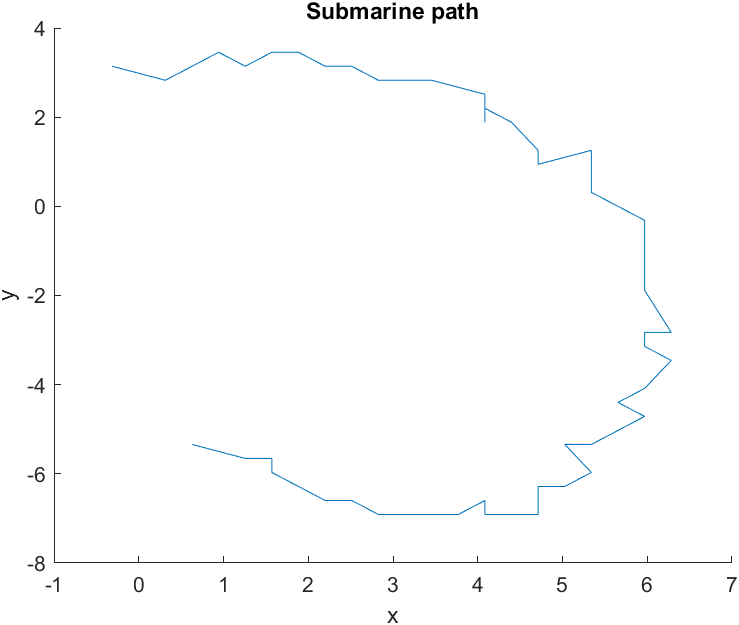
\includegraphics[width=0.9\linewidth]{path_xy}    	
		\caption{Aerial view}
	\end{subfigure}%
	\begin{subfigure}{.5\textwidth}
		\centering
		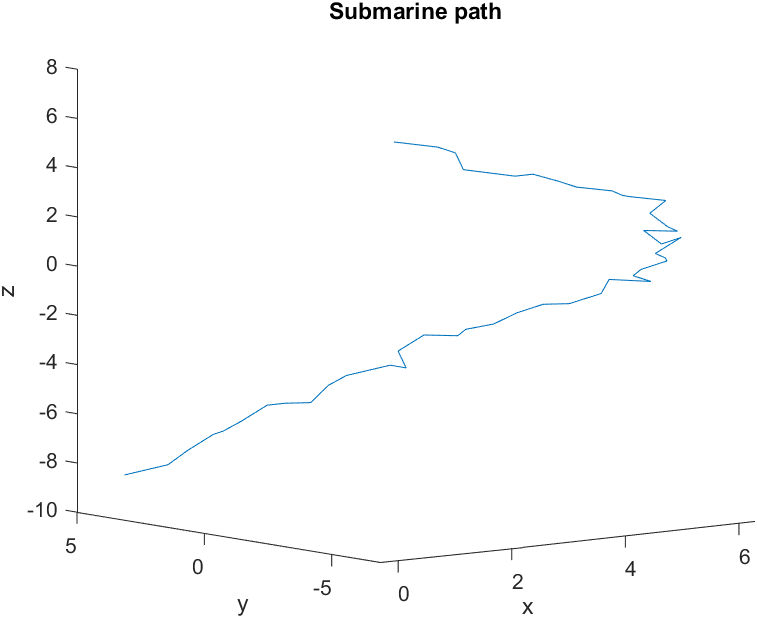
\includegraphics[width=0.9\linewidth]{path_xyz}    	
		\caption{3-D view}
	\end{subfigure}
	\caption{Estimated submarine trajectory in Puget Sound over 48 hours.}
	\label{fig:trajectory}
\end{figure}





% References
\printbibliography

% Appendices
\begin{appendices}

% MATLAB Functions
\section{MATLAB Functions}
\begin{itemize}
    \item \texttt{y = linspace(x1,x2,n)} returns a row vector of \texttt{n} evenly spaced points between \texttt{x1} and \texttt{x2}. 
    \item \texttt{[X,Y] = meshgrid(x,y)} returns 2-D grid coordinates based on the coordinates contained in the vectors \texttt{x} and \texttt{y}. \text{X} is a matrix where each row is a copy of \texttt{x}, and \texttt{Y} is a matrix where each column is a copy of \texttt{y}. The grid represented by the coordinates \texttt{X} and \texttt{Y} has \texttt{length(y)} rows and \texttt{length(x)} columns.  
    
    \item \texttt{ut = fftn(u)} Implements the N-Dimensional Fast Fourier Transform. When passed a 3-dimensional matrix \texttt{u}, it applies the 1-D transform along each of the 3 dimensions. Each 1-D transform outputs first the nonnegative bins in increasing order, then the negative bins in increasing order.
    
    \item \texttt{u = ifftn(ut)} Implements the N-Dimensional Inverse Fast Fourier Transform. Just like the previous bullet, when passed a 3-dimensional matrix \texttt{ut}, it applies the 1-D inverse transform along each of the 3 dimensions, outputting first the nonnegative bins in increasing order, then the negative bins in increasing order.
    
    \item \texttt{us = fftshift(ut)} Rearranges the output of \texttt{ut = ffshift(u)} so that the bins are all sorted increasing order.
\end{itemize}

% MATLAB Codes
\section{MATLAB Code}
\inputminted{matlab}{submarine_hunting.m}

\end{appendices}

\end{document}